{
\begin{table}[th]
\begin{center}
\begin{center}
\begin{tabular}{ c | c | c | c | c | c }\normalsize
\normalsize Workload & \normalsize Read & \normalsize Update & \normalsize Scan & \normalsize Insert & \normalsize R\&U \\
\hline
A & 50\% & 50\% & - & - & - \\
B & 95\% & 5\% & - & - & - \\
C & 100\% & - & - & - & - \\
D & 95\% & - & - & 5\% & - \\
E & - & - & 95\% & 5\% & - \\
F & 50\% & - & - & - & 50\% \\
\end{tabular}
\end{center}
\caption[YCSB Workload Properties.]
{
YCSB Workload Properties.
The percentage of operations in each YCSB workload. 
R\&U stands for Read and Update.
}
\label{tbl-ycsb}
\end{center}
\end{table}
}
{
\begin{figure*}[th]
\begin{center}
\centerline{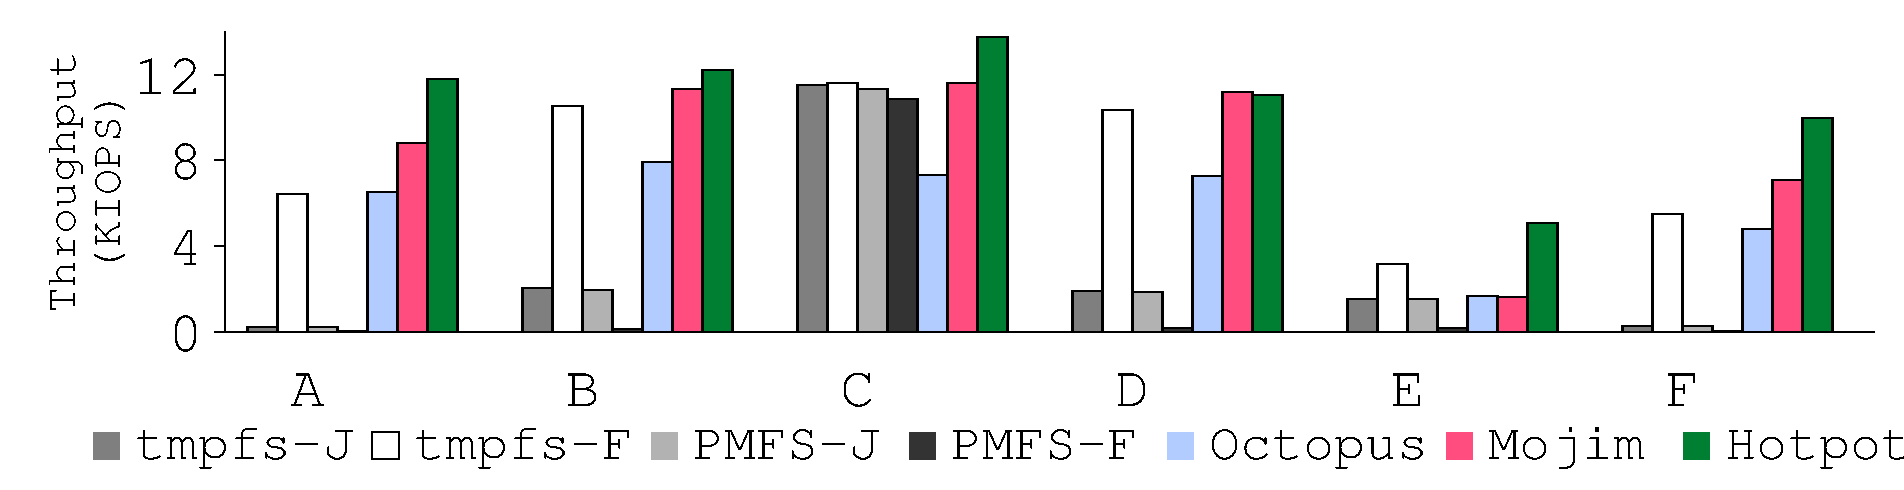
\includegraphics[width=\textwidth]{hotpot/Figures/g_plot_YCSB_run_throughput.pdf}}
\caption[YCSB Workloads Throughput.]{YCSB Workloads Throughput.}
\label{fig-ycsbrun}
\end{center}
\end{figure*}
}
